\chapter{提案手法}
既存手法であるGTCNNにおいて, コンテクスト抽出を担うGTLはU-Netをベースに設計されている. 本論文ではGTLの各層にCNN以上にコンテクスト抽出性能の優れたTransformerを組み込んだ手法, SAGTCNN (Self-Attention GTCNN) を提案する. Transformerを挿入する場所を変更したいくつかのバージョンを提案し, それらの性能を比較する. 実験を通して, Transformerのヘッドの数は1としている. 提案手法はGTLを変更した以外は従来のGTCNNのアーキテクチャを踏襲している. またパラメータサイズの比較は表\ref{tab:p_size}にて示している.

\section{SAGTCNN-S4}
SAGTCNN-S4は図\ref{fig:GTL_S4}のような構造になっている. 青い枠の部分が従来手法に変更を加えたところである. 従来手法では全ての層がCNN Blockで形成されていたがSAGTCNN-S4では4段目をSA Blockに変更しているところに特徴がある. さらに, プーリングよるダウンサンプリングを畳み込みで行うようにし, バイリニアでのアップサンプリングを畳み込みで行うように変更した. SA Blockは畳み込みを2度行うD-conv層とAttention層の2層からなっている. Transformerは画像のスケールが大きくなるほど計算量が増大するため, スケールの小さい4段目でTransformerを用いることで計算量の増大を防いでいる. 

\begin{figure}[htbp]
\centering
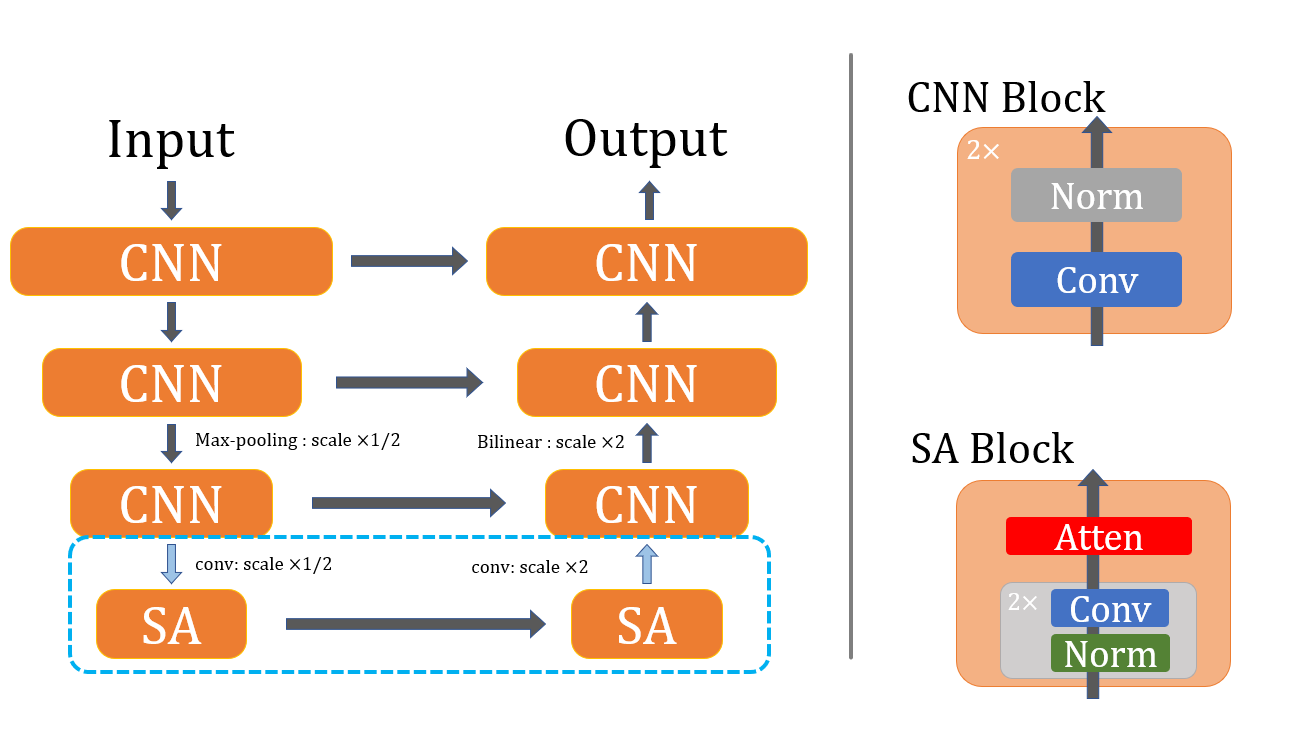
\includegraphics[scale=0.4]{figures/GTL_TS4.png}
\caption{SAGTCNN-S4のGTLのアーキテクチャ \label{fig:GTL_S4}}
\end{figure}

\newpage
\section{SAGTCNN-M}
SAGTCNN-Mでは本来なんの処理もなされていなかったミドル層にTransformerを追加した. アーキテクチャは図\ref{fig:GTL_M}の通りである. ミドル層は他の層と比べてスケールが最も小さくTransformerの処理も最も軽いため, 効率的にノイズ除去性能の向上を行える可能性があり実験を行った.

\begin{figure}[htbp]
\centering
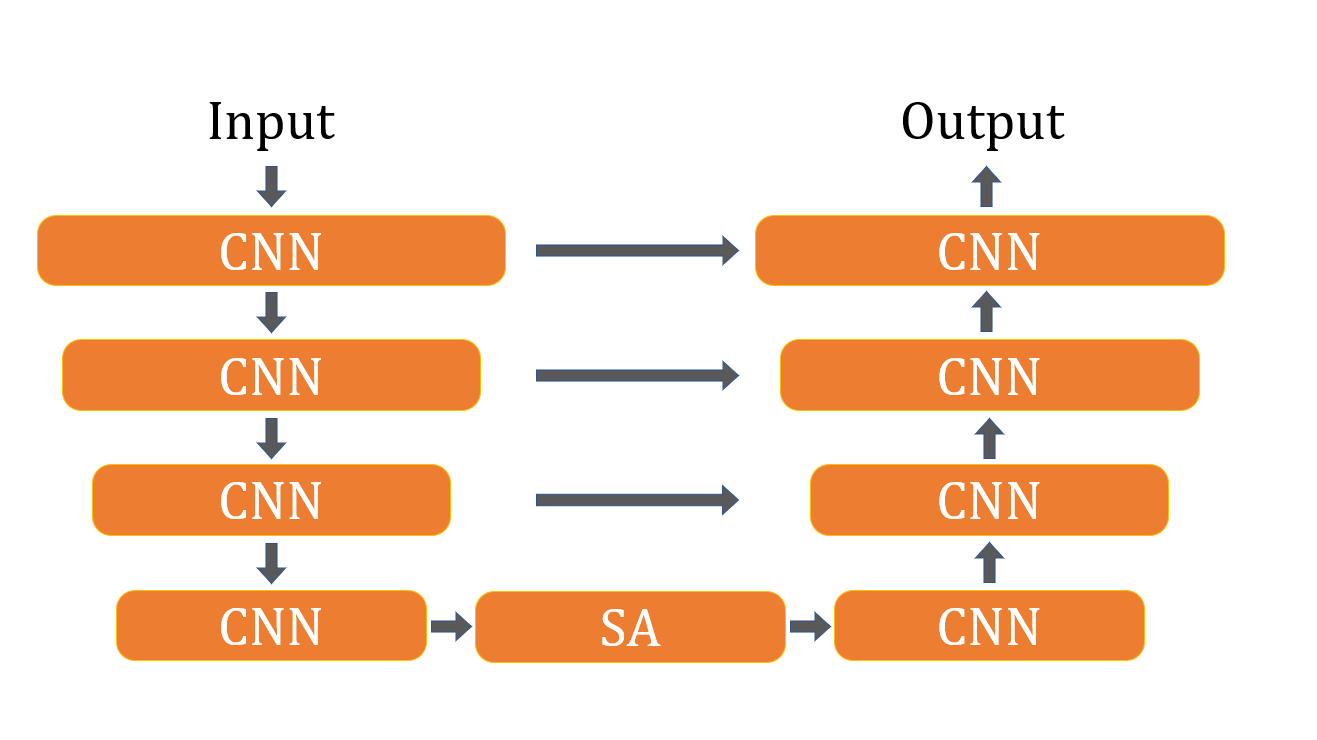
\includegraphics[scale=0.3]{figures/GTL_M.png}
\caption{SAGTCNN-MのGTLのアーキテクチャ \label{fig:GTL_M}}
\end{figure}

\section{SAGTCNN-S4M}
SAGTCNN-S4およびSAGTCNN-Mを合わせた手法で, Transformerを4段目とミドル層に挿入した. 計算量およびパラメータサイズは他の手法より大きくなる. 

\begin{table}[htbp]
\centering
\caption{パラメータサイズの比較 \label{tab:p_size}}
 \begin{tabular}{|c|c|c|c|}
 \hline
 GTCNN & SAGTCNN-S4 & SAGTCNN-M & SAGTCNN-S4M \\ \hline \hline 
   $\mathbf{851k}$ & 996k & 1,016k & 1,161k \\ \hline
 \end{tabular}
\end{table}